% !TEX root = ../Lazcorreta.Tesis.tex

\ABIERTO%

La obtención, almacenamiento y distribución de grandes cantidades de datos está al alcance de todo el mundo gracias a la \textsl{Informática}, la \textsl{Telecomunicación} y el resto de ciencias que han impulsado el crecimiento de ambas. Entidades de todo tipo (personas físicas o jurídicas, empresas públicas y privadas, organizaciones de diversos ámbitos\ldots) pueden disponer con facilidad de equipos informáticos y telemáticos capaces de recoger, almacenar y distribuir información de forma masiva. Esto las convierte en entidades propietarias de colecciones con enormes cantidades de datos en crudo. Si nos quedamos con estas aportaciones estaremos hablando de un problema de \textsl{infoxicación}, la "`incapacidad de llevar a cabo un análisis eficiente de gran cantidad de información"'.
%NOTA DISERTACIÓN: RAW (crudo en inglés) es el formato digital de imagen, no estándar, que recoge la información capturada por los sensores de imagen de una cámara digital. Son datos sin procesar a los que no se les ha aplicado aún ningún algoritmo de "`mejora"' de los datos a almacenar para ser capaces de comprenderlos (una imagen RAW no se visualiza en cualquier pantalla, una JPEG sí).

Cada día surgen nuevos dispositivos capaces de medir, almacenar y distribuir nuevos datos añadiéndolos o combinándolos con los que ya tenemos, lo que redunda en el exceso de información cruda de que disponemos. Esto acrecentaría el problema planteado si no hubiera sido tratado desde todas las ciencias existentes (Arte, Medicina, Historia, Informática, Investigación Operativa\ldots). Desde hace más de 4 décadas todos los investigadores se han encontrado con grandes y crecientes colecciones  de datos en crudo y con la necesidad de extraer de ellos, de forma eficiente, parte del conocimiento que contienen. De aquí surgen múltiples estudios sobre cómo transformar tanta información dinámica en conocimiento.

La globalización de la \www\ (WWW) no ha hecho más que acrecentar el problema. Cada día más con la aparición y popularización de sistemas de comunicación inalámbrica que permiten comunicar fácilmente dispositivos de proceso, almacenamiento y visualización de datos entre sí, sea cual sea su ubicación. La \WWW\ es el medio de generación, almacenamiento y distribución masiva de datos más representativo. Ya en~\cite*{Etzioni-TheWWWQuagmireOrGoldMine-1996} Etzioni se preguntaba si la enorme cantidad de información que estaba generando la \WWW\ en su época era un lodazal o una mina de oro. Se estaban adaptando las bases de la \dm\ (DM) a la \wm\ (WM). Para comprender el comportamiento de los usuarios de la \WWW\ se podían buscar \patrones entre los datos que genera su propio uso y facilitar con ellos la obtención de los objetivos de cada usuario al navegar por la web, aparecía la \wum\ (\WUM).
%desde tres perspectivas distintas: \wum (\WUM por sus siglas en inglés), \wsm (\WSM por sus siglas en inglés) y \wcm (\WCM por sus siglas en inglés).
Hoy en día sabemos que la \WWW\ es una mina de oro, pero hay que saber convertir la información que contienen los millones de datos que genera a diario en conocimiento capaz de ser utilizado por los medios de que dispone cada persona en muchas de sus tareas cotidianas.

\begin{figure}[htbp]
	\centering
  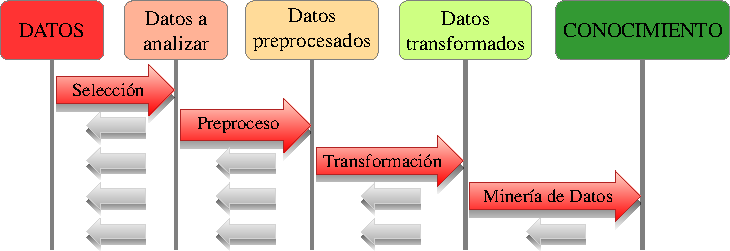
\includegraphics[width=.85\textwidth]{WorkFlow}
  \caption{Proceso \KDD}
\label{fig:resumen-fasesProcesoKDD}
\end{figure}

En la misma época estaba emergiendo con fuerza el \kdd (KDD), "`el proceso no trivial de identificar \patrones de datos válidos, novedosos, potencialmente útiles y comprensibles"' según~\citet{FayyadPiatetskySmyth-FromDataMiningToKnowledgeDiscoveryInDatabases-1996}. El proceso es puramente científico: la materia prima es una colección de datos a la que se le aplican cinco tareas secuenciales y recursivas (con retroalimentación) y cuyo producto final es el conocimiento. \citeauthor*{FayyadPiatetskySmyth-FromDataMiningToKnowledgeDiscoveryInDatabases-1996} inciden en la diferencia entre \dm y \kdd, la primera es una tarea de la segunda (ver figura~\ref{fig:resumen-fasesProcesoKDD}). Sin embargo algunos autores las confunden debido a que la recursividad del proceso de \KDD hace que la \DM tenga que ser ajustada y reutilizada con lo que podría considerarse un sub-proceso completo de adquisición de conocimientos.

Aunque he mencionado que la \WUM es una derivación de la \DM realmente es un proceso específico y completo de \KDD ya que se ha de estudiar qué datos se utilizarán de entre los disponibles, se han de preprocesar adecuadamente, transformar de modo que puedan ser analizados mediante \DM y finalmente evaluar los resultados, todo ello de forma recursiva siempre que en el proceso aparezcan resultados intermedios que lo aconsejen.

Uno de los grandes paradigmas de la ciencia es "`divide y vencerás"', y es perfectamente aplicable a cualquier proceso de \KDD. Cada investigador se centra en su especialidad para mejorar un pequeño aspecto de la ciencia. En mi caso he querido aportar mis conocimientos sobre algoritmia (matemáticas e informática), análisis de datos (estadística y matemáticas) y programación (informática) por lo que tras estudiar el estado del arte sobre el proceso completo de la \wum decidí dedicar mi investigación a la \dm.

Nuestros primeros trabajos se centraron en la \indice{Personalización de la Web}~\citep{Anderson-AMachineLearningApproachToWebPersonalization-2002}, concretamente en el análisis de los \srws (\SRW) a través de la \wum, introduciendo nuevos métodos para la fase de \dm que permitieran aliviar los problemas ya sugeridos por otros investigadores. La publicación en congresos de nuestros trabajos nos ofreció la oportunidad de compartir estas propuestas con colegas de especialidades afines o complementarias e ir creciendo en conocimientos generales sobre el tema. Tras analizar las primeras tareas del \KDD aplicadas al estudio del uso de la web llegamos a conclusiones similares al de resto de investigadores respecto a las primeras tareas del proceso: los datos iniciales se han seleccionar y preprocesar adecuadamente (fijando ciertos parámetros de forma empírica) y transformar en \sns.

Nuestra primer propuesta fue el uso de \grafos para representar las \sns y analizar el uso de la web por parte de los internautas. Los \grafos permiten estudiar las \secuencias de páginas producidas por los usuarios en sus \sns, de las que podemos extraer tanto la co-ocurrencia de páginas en una misma sesión como el orden en que fueron visitadas. Aunque este camino parecía adecuado su tratamiento sobre colecciones de datos muy grandes desbordaba las capacidades de las máquinas usadas para nuestra investigación.

En nuestra segunda propuesta decidimos cambiar el tratamiento dado a las \sn, considerándolas como colecciones de \transacciones, grupos de páginas recorridos en la misma sesión sin importar el orden en que fueron visitadas, reduciendo las dimensiones del problema para aliviar la carga de procesamiento y almacenamiento de los datos a tratar. El trabajo de \citet{AgrawalSrikant-FastAlgorithmsForMiningAssociationRules-1994} nos abrió nuevos caminos con la introducción del algoritmo \apriori, un elegante algoritmo capaz de encontrar gran cantidad de \ARs entre los datos que estábamos manejando. Lo incorporamos a nuestro trabajo porque su sencillez daba mucho juego y podíamos adaptarlo a nuestro objetivo: encontrar \patrones de navegación de los usuarios de un sitio web para su personalización~\citep{BorgesLevene-DataMiningOfUserNavigationPatterns-1999}. Los resultados obtenidos en esta fase se exponen en el capítulo~\ref{chap:SRW}.

Las \ARs son una descripción de las co-ocurrencias existentes entre los diferentes ítems de una \transaccion (las diferentes páginas visitadas en un sitio web durante una \sn, en nuestro caso). Conceptualmente están más cercanas a la Estadística Descriptiva que a la \DM pero en la práctica permiten abordar el análisis de inmensas colecciones de \transacciones por lo que han sido abordadas desde el punto de vista informático debido principalmente al llamado \dilemaIR, que postula que los ítems menos frecuentes en el análisis pueden hacer inviable el estudio completo de la colección de datos debido a problemas de desbordamiento y falta de recursos. Este dilema nos preocupaba pues la catalogación de un ítem como "`raro"' sólo dependía del número de veces que aparecía en las \transacciones (su frecuencia absoluta o \soporte según el lenguaje de las \ar) y no de otros factores que podrían ser más significativos.

En el capítulo~\ref{chap:arm} planteamos dos modificaciones al algoritmo \apriori original. Los datos nos proporcionan información sobre \textsl{"`qué hace"'} el usuario, las \ars nos pueden dar información sobre \textsl{"`cómo lo hacen"'}. Esto nos sugirió la primera de nuestras aportaciones abordando una búsqueda de relaciones entre las \ars encontradas entre los datos analizados con la intención de agrupar a los usuarios de un sitio web en función de \textsl{"`qué reglas cumplen"'} y no únicamente en función de \textsl{"`qué páginas visitan"'}. De aquí surgió la única publicación que tengo hasta la fecha en una revista científica de impacto dando mucha más visibilidad a mi aportación que la obtenida en los diferentes congresos en que hemos expuesto nuestras ideas (véase~\ref{sec:nuestro-Torwards-2008}). Sin embargo esta solución incrementaba el \dilemaIR.

La segunda aportación presentada en este capítulo proponía una solución sencilla para tratar este dilema en situaciones en que los ítems menos frecuentes pueden ser de importancia, concretamente en su aplicación a los \SRW. Se trataba de usar las \ROPs (junto a las \ARs) de modo que un \srw pudiera no sólo sugerir al usuario las páginas más relacionadas con aquellas que ya ha visitado si no que también pudiera sugerirle páginas menos frecuentes posiblemente relacionados con sus objetivos.

En el capítulo~\ref{chap:conclusiones-y-trabajo-futuro} se vuelven a tomar estos temas pues pueden ser mejorados utilizando técnicas estadísticas, de \clasificacion y de investigación operativa que no se han podido abordar en esta tesis.

El \dilemaIR seguía preocupándonos. Aunque trabajemos con mucha información simultáneamente los actuales sistemas informáticos han de ser capaces de ofrecer información válida sobre todos los ítems de una colección de \transacciones. Hay diversos estudios sobre las limitaciones de la tecnología y algoritmia actual para afrontar un estudio completo de una colección grande de \transacciones [libro que no consigo y limita el análisis de mushroom y chess], hay trabajos que ayudan a determinar qué ítems raros deben ser analizados, el dilema se aborda desde muchas perspectivas aplicando distintas técnicas del tipo "`divide y vencerás"'. Pero si no nos esforzamos en incluir en un único proceso la información que contienen los ítems raros el conocimiento adquirido tendrá menos calidad y, sobre todo, no se podrán estudiar a fondo problemas tan actuales como las enfermedades raras, nuevos métodos de fraude\ldots

La mayor aportación de esta tesis se expone en el capítulo~\ref{chap:clasificacion}, donde abordamos el estudio de ciertas colecciones de \transacciones extensamente utilizadas por la comunidad científica, los \catalogos y las muestras que se obtienen a partir de su estructura. En el [libro que...] ponen límite a la información que se puede analizar en colecciones de este tipo, como \mushroom. Expondremos que no debemos renunciar a ningún tipo de información ofrecida por ese fichero, podemos aprovechar la rigidez de su estructura para reducir drásticamente el número de elementos a analizar. Al aplicar la reducción propuesta podremos obtener todas las \ARs contenidas en la colección de \transacciones utilizando los algoritmos ya conocidos sobre esta materia.

Para terminar esta investigación proponemos el uso de estructuras informáticas adaptadas a la flexibilidad y agilidad necesaria en \dm proponiendo el uso de \CCs\ldots


%El presente trabajo comenzó con la idea de aplicar el proceso de \KDD a la personalización de la web. Y entre las tareas que ello involucra las que se adaptaban mejor a mi son perfil aquellas con aspectos matemáticos, estadísticos e informáticos. Una de estas tareas es la \dm (DM), que algunos autores confunden con la \KDD. En el proceso de \KDD interviene la obtención de datos, decisiones estratégicas de almacenamiento, selección de objetivos para los que se guardan los datos, selección de los datos que van a ser analizados\ldots y su \textsl{minado} usando técnicas de \dm.
%
%
%
%
%
%Presentaban buenas propuestas sobre su relación con la \dm, algo cada vez más evidente por el vertiginoso aumento de capacidades de los equipos informáticos utilizados por los investigadores. Aumento que no cesa hoy en día y que permite buscar soluciones alternativas a las planteadas hasta la fecha.
%
%No se puede analizar toda la información disponible, pero podemos crear \patrones o modelos que expliquen gran parte del conocimiento escondido en dicha información. Si estos \patrones son correctos podremos conocer características imposibles de medir directamente, construyéndolas a partir de la información que hemos sido capaces de medir directa o indirectamente.
%
%
%
%
%
%Hoy es mucho mayor el problema en cuanto a cantidad de información, pero se han analizado multitud de soluciones desde la perspectiva de la \kdd (KDD), la extracción de conocimiento útil y previamente desconocido de una ingente cantidad de datos ya disponibles.% Es el nombre que recibe actualmente la transformación de información (experiencia) en conocimiento (ciencia) mediante el uso de la informática y la telemática.
%
%
%
%
%
%Esta tesis se centra en el análisis y desarrollo de algoritmos adaptados a la extracción de conocimiento de grandes colecciones de datos (muy usadas) utilizando recursos fácilmente disponibles.
%
%Este trabajo se centra en una pequeña parte del proceso de \KDD
%
%
